\documentclass[10pt]{article}

\usepackage{spheric}
%%%TITLE
\title{SPH numerical investigation of oscillating characteristics of hydraulic jumps at an abrupt drop}
\date{}

%%AFFILIATIONS
\author[1]{Diana De Padova}
\author[1]{Michele Mossa}
\author[2]{Stefano Sibilla}

\affil[1]{Department of Civil, Environmental, Building Engineering and Chemistry, Technical University of Bari, Italy}
\affil[2]{Department of Civil Engineering and Architecture, University of Pavia, Italy}

%%DOCUMENT
\begin{document}

\maketitle

%\SelectedTopics{}

%%PLEASE PUT YOUR ABSTRACT HERE
\begin{abstract}
This paper shows the results of the SPH modelling of the transition from supercritical to subcritical flow at an abrupt drop based on the laboratory experiments by Mossa et al. \cite{mossa2003tailwater}. At an abrupt drop the transition from supercritical to subcritical flow is characterised by several flow patterns depending upon the inflow and tailwater flow conditions. SPH simulations are obtained by a pseudo-compressible XSPH scheme with pressure smoothing; turbulent stresses are represented either by an algebraic mixing- length model, or by a two-equation $k-\varepsilon$ model. The numerical model is applied to analyze the occurrence of oscillatory flow conditions between two different jump types characterised by quasi-periodic oscillation, and the results are compared with experiments performed at the hydraulics laboratory of Bari Technical University. Figure \ref{fig:14-1} shows an example of an oscillation cycle between a B-type jump (a,c) and a wave jump (b,d). The purpose of this paper is to obtain a deeper understanding of the physical features of a flow which is in general difficult to be reproduced numerically, owing to its unstable character. In particular, relying on previous SPH analyses of vorticity-dominated flows \cite{de2016sph}, vorticity fields, velocity, water depth and pressure spectra downstream of the jump (fig. \ref{fig:14-2}), and velocity and pressure cross-correlations can be computed and analysed.

\begin{figure}[!htb]
\begin{minipage}[b]{0.42\linewidth}
\centering
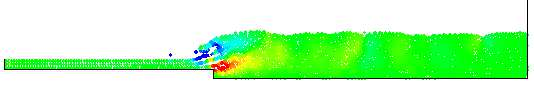
\includegraphics[width=0.9\textwidth]{14-11.png} (a)\\
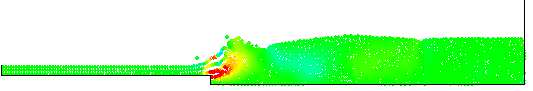
\includegraphics[width=0.9\textwidth]{14-12.png} (b)\\
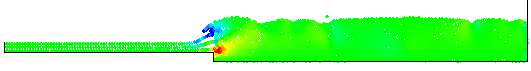
\includegraphics[width=0.9\textwidth]{14-13.png} (c)\\
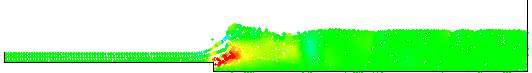
\includegraphics[width=0.9\textwidth]{14-14.png} (d)
\caption{Instantaneous vorticity fields in the SPH simulation: a) $t=15$ s; b) $t=21$ s; c) $t=26$ s; d) $t=30$ s.}\label{fig:14-1}
\end{minipage}
\begin{minipage}[b]{0.05\linewidth}
~
\end{minipage}
\begin{minipage}[b]{0.5\linewidth}
\centering
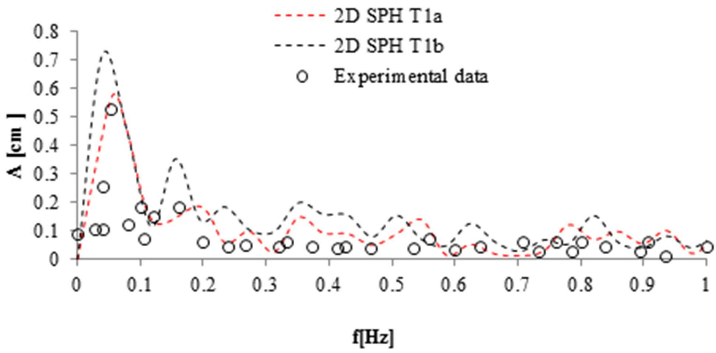
\includegraphics[width=\textwidth]{14-2.png}
\caption{Amplitude spectra of pressure fluctuations under the jump for SPH simulations with ML turbulence model (T1a), with $k-\varepsilon$ model (T1b) and experiments}\label{fig:14-2}
\end{minipage}
\end{figure}

\end{abstract}

%%THE END OF ABSTRACT

\addbib

\end{document}
